\documentclass[a4paper,11pt]{article}

% set up sensible margins (same as for cssethesis)
\usepackage[paper=a4paper,left=30mm,right=30mm,top=25mm,bottom=25mm]{geometry}
\usepackage{natbib} % Use the natbib bibliography and citation package
\usepackage{setspace} % This is used in the title page
\usepackage{graphicx} % This is used to load the crest in the title page
\usepackage{physics} % Used for \abs

% non-template packages
\usepackage{paralist}
\usepackage{multicol}
\usepackage{caption}
\usepackage{tabularx, booktabs}
\newcolumntype{Y}{>{\centering\arraybackslash}X}
\usepackage{listings}
\lstset{
	numbers=left, 
	numberstyle=\small, 
	numbersep=8pt, 
	frame = single, 
	language=Python, 
	framexleftmargin=17pt}

\usepackage{tikz}
\usepackage{smartdiagram}

\usepackage[font={small,it}]{caption}
\usepackage{hyperref}
\usepackage{xcolor}
\usepackage{lscape}
\hypersetup{
	colorlinks,
	linkcolor=teal,
	citecolor=teal,
	urlcolor=blue
}

\usepackage[english]{babel}
\usepackage{blindtext}

%tikz stuff
\usepackage{tikz}
\usetikzlibrary{shapes, arrows, trees}
\tikzstyle{decision} = [diamond, draw, fill=green!20, text width=4.5em, text badly centered, node distance=3cm, inner sep=0pt]
\tikzstyle{block} = [rectangle, draw, fill=yellow!20, text width=3cm, text centered, rounded corners, minimum height=4em]
\tikzstyle{line} = [draw, -latex']
\tikzstyle{straight} = [draw]


\usepackage{array}
\newcolumntype{L}[1]{>{\raggedright\let\newline\\\arraybackslash\hspace{0pt}}m{#1}}
\newcolumntype{C}[1]{>{\centering\let\newline\\\arraybackslash\hspace{0pt}}m{#1}}
\newcolumntype{R}[1]{>{\raggedleft\let\newline\\\arraybackslash\hspace{0pt}}m{#1}}

\usepackage{float}

%\hypersetup{
%	colorlinks,
%	linkcolor={red!50!black},
%	citecolor={blue!50!black},
%	urlcolor={blue!80!black}
%}

\begin{document}
	
% Set up a title page
\thispagestyle{empty} % no page number on very first page
% Use roman numerals for page numbers initially
\renewcommand{\thepage}{\roman{page}}

\begin{spacing}{1.5}
	\begin{center}
		{\Large \bfseries
			School of Computer Science (BICA) \\
			Monash University}
		
		
		\vspace*{30mm}
		
		
\includegraphics[width=5cm]{graphics/MonashCrest.pdf}
		
		\vspace*{15mm}
		
		{\large \bfseries
			Literature Review, 2017
		}
		
		\vspace*{10mm}
		
		{\LARGE \bfseries
			Improving cooperative pathfinding using a path oracle
		}
		
		\vspace*{20mm}
		
		{\large \bfseries
			Phillip Wong
			
			\vspace*{20mm}
			
			
			Supervisors: \parbox[t]{50mm}{Daniel Harabor,\\Pierre Le Bodic}
		}
		
	\end{center}
\end{spacing}

\newpage

\tableofcontents

\newpage
% Now reset page number counter,and switch to arabic numerals for remaining
% page numbers 
\setcounter{page}{1}
\renewcommand{\thepage}{\arabic{page}}



\section{Introduction}
The order picking process is the number one expense in the operating cost of warehouse systems \cite{de2007design}. This project will look at warehouse automation, whereby the order-picking process is performed by automated vehicles. In particular we will we will be exploring Kiva systems which employs warehouse automation. More detail about Kiva systems is provided in Section~\ref{sec:background}.

% What
When improving on the part-to-picker systems, we look at the system as a Multi-agent pathfinding (MAPF) problem. 

% How
These include: introducing an intermediate dropping zone, optimizing order processing and adding the capability for robots to maneuver under storage pods.

% Where
The results of this project will help identify how we should position storage and picking stations in a warehouse. Additionally, we will be looking at developing a MAPF method which uses a pre-computed path oracle.
\section{Background} \label{sec:background}


\section{Multi-agent Pathfinding}
Multi-agent pathfinding (MAPF) involves finding a path for every agent to their goal. Warehouse Automation is commonly modeled on an orthogonal undirected grid \cite{TODO}. Formally defining this, we look at $k$ agents on a graph $G = (V, E)$ where V is the set of vertices and E is the set of edges within the graph.


\begin{figure}[h]
	\centering
	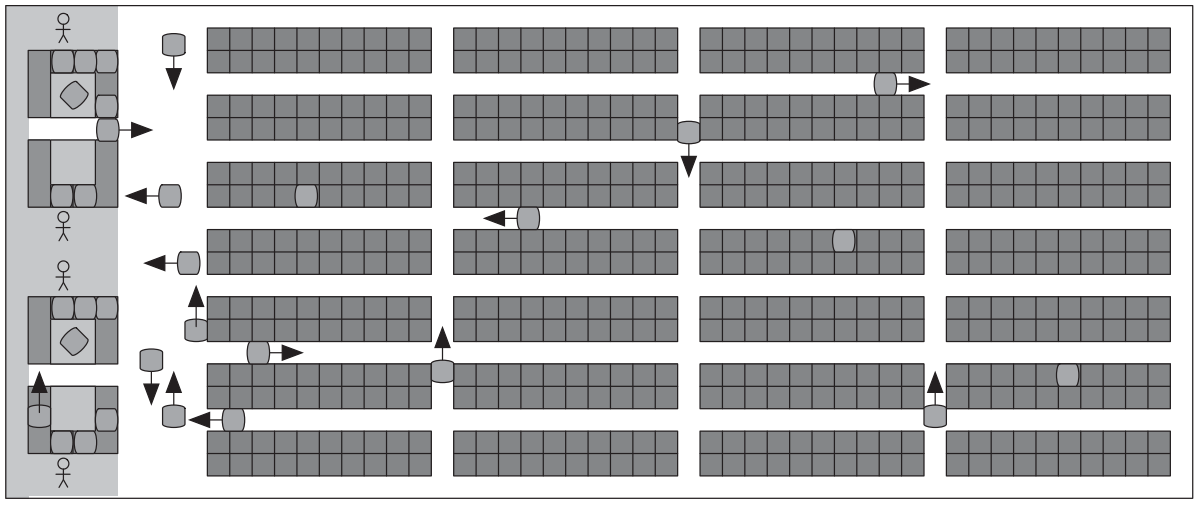
\includegraphics[width=0.9\textwidth]{graphics/kivasystemlayout}
	\caption{A Small Region of a Kiva Layout (\cite{wurman2008coordinating}). Picking stations located on the left and storage pods laid out in rows.}
	\label{kivalayout1}
\end{figure}

Within MAPF, we are focusing on an optimal solution. The following sections will focus on optimal MAPF algorithms as well as suboptimal variants of these algorithms.

\section{Conflict-based Search}
The state-of-the-art in MAPF, Conflict-based search is 

\section{Other optimal algorithms}
ICTS

\section{Mixed Integer Programming}
Mixed-integer programming (MIP) is an optimization technique that looks at an objective function which is subject to a list of constraints.


\section{Other reduction-based techniques}
Answer set programming?

\section{Other areas in Warehouse Automation}
Warehouse layout?

Order scheduling?

Drive allocation?

\section{Conclusion}


\bibliographystyle{dcu}
\bibliography{bibliography}
	
\end{document}
